\documentclass[
	% -- opções da classe memoir --
	12pt,                   % tamanho da fonte
	openany,                % capítulos começam em sequência
	twoside,                % para impressão em verso e anverso. Oposto a oneside
	a4paper,                % tamanho do papel. 
	% -- opções da classe abntex2 --
	%chapter=TITLE,         % títulos de capítulos convertidos em letras maiúsculas
	%section=TITLE,         % títulos de seções convertidos em letras maiúsculas
	%subsection=TITLE,      % títulos de subseções convertidos em letras maiúsculas
	%subsubsection=TITLE,   % títulos de subsubseções convertidos em letras maiúsculas
	% -- opções do pacote babel --
	english,                % idioma adicional para hifenização
	%french,                % idioma adicional para hifenização
	%spanish,               % idioma adicional para hifenização
	brazil                  % o último idioma é o principal do documento
	]{abntex2}

% ---------------------
% Pacotes OBRIGATÓRIOS
% ---------------------
\usepackage{lmodern}            % Usa a fonte Latin Modern			
\usepackage[T1]{fontenc}        % Selecao de codigos de fonte.
\usepackage[utf8]{inputenc}     % Codificacao do documento (conversão automática dos acentos)
\usepackage{lastpage}           % Usado pela Ficha catalográfica
\usepackage{indentfirst}        % Indenta o primeiro parágrafo de cada seção.
\usepackage{color}              % Controle das cores
\usepackage{graphicx,graphicx}  % Inclusão de gráficos
\usepackage{epsfig,subfig}      % Inclusão de figuras
\usepackage{microtype}          % Melhorias de justificação
\usepackage{csvsimple}          % Importar arquivos csv como tabelas
% ---------------------
		
% ---------------------
% Pacotes ADICIONAIS
% ---------------------
\usepackage{amsmath,amssymb,mathrsfs}  % Comandos matemáticos avançados 
\usepackage{algpseudocode,algorithm}   % Para poder adicionar algoritmos
\usepackage{setspace}                  % Para permitir espaçamento simples, 1 1/2 e duplo
\usepackage{verbatim}                  % Para poder usar o ambiente "comment"
\usepackage{tabularx}                  % Para poder ter tabelas com colunas de largura auto-ajustável
\usepackage{afterpage}                 % Para executar um comando depois do fim da página corrente
\usepackage{url}                       % Para formatar URLs (endereços da Web)
% ---------------------

% ---------------------
% Pacotes de CITAÇÕES
% ---------------------
\usepackage[brazilian,hyperpageref]{backref} % Paginas com as citações na bibl
\usepackage[alf]{abntex2cite}                % Citações padrão ABNT (alfa)
%\usepackage[num]{abntex2cite}               % Citações padrão ABNT (numericas)
% ---------------------

% Configura fonte serifada para títulos
\renewcommand{\ABNTEXchapterfont}{\rmfamily}

% Configura citação de algoritmo
\makeatletter
\renewcommand{\ALG@name}{Algoritmo}
\makeatother
\newcommand{\algorithmautorefname}{Algoritmo}

% Permite chamar um método dentro de outro método em algoritos
\MakeRobust{\Call}

% Configurações de CITAÇÕES para abntex2
% --- 
% CONFIGURAÇÕES DE PACOTES
% --- 

% ---
% Configurações do pacote backref
% Usado sem a opção hyperpageref de backref
\renewcommand{\backrefpagesname}{Citado na(s) página(s):~}
% Texto padrão antes do número das páginas
\renewcommand{\backref}{}
% Define os textos da citação
\renewcommand*{\backrefalt}[4]{
	\ifcase #1 %
		Nenhuma citação no texto.%
	\or
		Citado na página #2.%
	\else
		Citado #1 vezes nas páginas #2.%
	\fi}%
% ---

% Inclusão de dados para CAPA e FOLHA DE ROSTO (título, autor, orientador, etc.)
% ---
% Informações de dados para CAPA e FOLHA DE ROSTO
% ---
\titulo{Este é o Título da Dissertação}
\autor{Autor da Dissertação}
\local{Santo André - SP}
\data{Xxxx de 20XX}
\orientador{Fulano Nome do Orientador}
\coorientador{Fulano Nome do Coorientador}
\instituicao{%
  Universidade Federal do ABC -- UFABC
  \par
  Centro de Engenharia, Modelagem e Ciências Sociais Aplicadas 
  \par
  Programa de Pós-Graduação em Engenharia da Informação}
\tipotrabalho{Dissertação (Mestrado)}
% O preambulo deve conter o tipo do trabalho, o objetivo,
% o nome da instituição e a área de concentração
\preambulo{\textbf{Dissertação de Mestrado} apresentada ao Programa de Pós-Graduação em Engenharia da Informação (área de concentração: Sistemas Inteligentes), como parte dos requisitos necessários para a obtenção do Título de Mestre em Engenharia da Informação.}
% ---

% Inclui Configurações de aparência do PDF Final
%  Configurações de aparência do PDF final
% NÃO ALTERAR!!!

% alterando o aspecto da cor azul
\definecolor{blue}{RGB}{41,5,195}

% informações do PDF
\makeatletter
\hypersetup{
     	%pagebackref=true,
		pdftitle={\@title}, 
		pdfauthor={\@author},
    		pdfsubject={\imprimirpreambulo},
	    pdfcreator={LaTeX with abnTeX2},
		pdfkeywords={abnt}{latex}{abntex}{abntex2}{trabalho acadêmico}, 
		colorlinks=true,       		% false: boxed links; true: colored links
    		linkcolor=blue,          	% color of internal links
    		citecolor=blue,        		% color of links to bibliography
    		filecolor=magenta,      		% color of file links
		urlcolor=blue,
		bookmarksdepth=4
} 
\makeatother
% --- 

% O tamanho da identação do parágrafo é dado por:
\setlength{\parindent}{1.3cm}

% Controle do espaçamento entre um parágrafo e outro:
\setlength{\parskip}{0.2cm}  % tente também \onelineskip

% ---------------------
% Compila o indice
% ---------------------
\makeindex
% ---------------------


%%%%%%%%%%%%%%%%%%%%%%%%%%%
%%  INICIO DO DOCUMENTO  %%
%%%%%%%%%%%%%%%%%%%%%%%%%%%
\begin{document}

% Retira espaço extra obsoleto entre as frases.
\frenchspacing

% ----------------------------------------------------------
% ELEMENTOS PRÉ-TEXTUAIS (Capa, Resumo, Abstract, etc.)
% ----------------------------------------------------------
\pretextual

% Capa
% ---
% Impressão da Capa
% ---
  \begin{capa}%
    \center
	\ABNTEXchapterfont\large\imprimirinstituicao
    \vfill
    \ABNTEXchapterfont\bfseries\LARGE\imprimirtitulo
    \vfill
	\ABNTEXchapterfont\large\imprimirautor
	\vfill
    \large\imprimirlocal \\ \large\imprimirdata
    \vspace*{1cm}
  \end{capa}
% ---


% Folha de rosto (o * indica que haverá a ficha bibliográfica)
\imprimirfolhaderosto*

% Imprimir Ficha Catalografica
% % ---
% Ficha Catalográfica
% ---
% Isto é um exemplo de Ficha Catalográfica, ou ``Dados internacionais de
% catalogação-na-publicação''. Você pode utilizar este modelo como referência. 
% Porém, talvez a biblioteca lhe fornece um PDF
% com a ficha catalográfica definitiva após a defesa do trabalho. Quando estiver
% com o documento, salve-o como PDF no diretório do seu projeto e substitua todo
% o conteúdo de implementação deste arquivo pelo comando abaixo:
%
% \begin{fichacatalografica}
%     \includepdf{fig_ficha_catalografica.pdf}
% \end{fichacatalografica}
\begin{fichacatalografica}
	\vspace*{\fill}					% Posição vertical
	\hrule							% Linha horizontal
	\begin{center}					% Minipage Centralizado
	\begin{minipage}[c]{12.5cm}		% Largura
	
	\imprimirautor
	
	\hspace{0.5cm} \imprimirtitulo  / \imprimirautor. --
	\imprimirlocal, \imprimirdata-
	
	\hspace{0.5cm} \pageref{LastPage} p. : il. (algumas color.) ; 30 cm.\\
	
	\hspace{0.5cm} \imprimirorientadorRotulo~\imprimirorientador\\
	
	\hspace{0.5cm}
	\parbox[t]{\textwidth}{\imprimirtipotrabalho~--~\imprimirinstituicao,
	\imprimirdata.}\\
	
	\hspace{0.5cm}
		1. Palavra-chave1.
		2. Palavra-chave2.
		I. Orientador.
		II. Universidade xxx.
		III. Faculdade de xxx.
		IV. Título\\ 			
	
	\hspace{8.75cm} CDU 02:141:005.7\\
	
	\end{minipage}
	\end{center}
	\hrule
\end{fichacatalografica}
% ---

% Inserir Folha de Aprovação
% ---
% Assinaturas
% ---
% Isto é um exemplo de Folha de aprovação, elemento obrigatório da NBR
% 14724/2011 (seção 4.2.1.3). Você pode utilizar este modelo até a aprovação
% do trabalho. Após isso, substitua todo o conteúdo deste arquivo por uma
% imagem da página assinada pela banca com o comando abaixo:
%
% \includepdf{folhadeaprovacao_final.pdf}
%
\begin{folhadeaprovacao}

  \begin{center}
    {\ABNTEXchapterfont\large\imprimirautor}

    \vspace*{\fill}\vspace*{\fill}
    \begin{center}
      \ABNTEXchapterfont\bfseries\Large\imprimirtitulo
    \end{center}
    \vspace*{\fill}

    \hspace{.45\textwidth}
    \begin{minipage}{.5\textwidth}
        \imprimirpreambulo
    \end{minipage}%
    \vspace*{\fill}
   \end{center}

 % Isso na versao final do trabalho!!!       
 % Trabalho aprovado. \imprimirlocal, 01 de janeiro de 2014:

   \assinatura{\textbf{\imprimirorientador} \\ Orientador}
   \assinatura{\textbf{Prof. Dr. Alexandre Donizeti Alves} \\ Convidado 1}
   \assinatura{\textbf{Prof. Dr. Thiago Ferreira Covões} \\ Convidado 2}

   \begin{center}
    \vspace*{0.5cm}
    {\large\imprimirlocal}
    \par
    {\large\imprimirdata}
    \vspace*{1cm}
  \end{center}

\end{folhadeaprovacao}
% ---


% Dedicatória
% ---
% Dedicatória
% ---
\begin{dedicatoria}
    \vspace*{\fill}
    \centering
    \noindent
    \textit{ À comunidade científica brasileira. } \vspace*{\fill}
\end{dedicatoria}
% ---

% Agradecimentos
% ---
% Agradecimentos
% ---
\begin{agradecimentos}
    Agradeço aos meus pais, que me deram apoio e incentivo. Sou grato também aos meus familiares, que compreenderam minha ausência pelo tempo dedicado aos estudos.

    Em especial, obrigado à Juliana, que não me deixou ser vencido pelo cansaço e me estimulou durante todos os anos da graduação.
\end{agradecimentos}
%% ---

% Epígrafe
% ---
% Epígrafe
% ---
\begin{epigrafe}
    \vspace*{\fill}
	\begin{flushright}
		\textit{``Não sei o que, \\
		          não sei o que,\\
                  não sei o que lá.''\\
		          (Autor Desconhecido)}
	\end{flushright}
\end{epigrafe}
% ---

% Resumo e Abstract
% ---
% RESUMOS
% ---

% RESUMO em português
\setlength{\absparsep}{18pt} % ajusta o espaçamento dos parágrafos do resumo
\begin{resumo}
   A análise de redes sociais permite...
   
   O estudo bibliométrico das coautorias...
   
   Neste projeto é proposto um método para a caracterização do impacto da Ciência da Computação nas demais áreas do conhecimento onde, a partir de currículos obtidos na Plataforma Lattes, são criadas redes de coautoria divididas em períodos, com pesquisadores sendo representados por nós e suas coautorias representadas por vértices. A relevância desse trabalho recai na possibilidade de explorar métricas topológicas medidas nas redes de coautoria para evidenciar o impacto que diferentes áreas do conhecimento recebem da Ciência da Computação, possibilitando que o método seja reproduzido em diferentes cenários.
    
    O método proposto para a identificação de coautorias realiza no máximo uma comparação entre qualquer par de publicações, produz o mesmo resultado independentemente da ordem de entrada e garante que o grafo de uma coautoria é sempre uma clique.

    \textbf{Palavras-chaves}: redes de coautoria. Ciência da Computação. Brasil.
\end{resumo}


% Lista de ilustrações
\pdfbookmark[0]{\listfigurename}{lof}
\listoffigures*
\cleardoublepage

% Lista de tabelas
\pdfbookmark[0]{\listtablename}{lot}
\listoftables*
\cleardoublepage

% Lista de algoritmos
\renewcommand{\listalgorithmname}{Lista de algoritmos}
\pdfbookmark[0]{\listalgorithmname}{loa}
\listofalgorithms
\cleardoublepage

% Lista de abreviaturas e siglas
% \begin{siglas}
%   \item[ABNT] Associação Brasileira de Normas Técnicas
%   \item[abnTeX] Normas para TeX
% \end{siglas}

% Lista de símbolos
% \begin{simbolos}
%   \item[$ \Gamma $] Letra grega Gama
%   \item[$ \Lambda $] Lambda
%   \item[$ \zeta $] Letra grega minúscula zeta
%   \item[$ \in $] Pertence
% \end{simbolos}

% Inserir o SUMÁRIO
\pdfbookmark[0]{\contentsname}{toc}
\tableofcontents*
\cleardoublepage

% ----------------------------------------------------------
% ELEMENTOS TEXTUAIS (Capítulos)
% ----------------------------------------------------------
\textual
% Elementos textuais com numeração arábica
\pagenumbering{arabic}
% Reinicia a contagem do número de páginas
\setcounter{page}{1}

% Inclui cada capitulo da Dissertação
\chapter[Introdução]{Introdução}

O número de pesquisas feitas em coautoria vêm aumentando no Brasil \cite{mena2014brazilian} e no mundo \cite{glanzel2003bibliometrics} em diferentes áreas do conhecimento, tanto entre áreas distintas quanto dentro de uma mesma área. Compreender a dinâmica dessas coautorias e medir o impacto\footnote{O termo impacto é subjetivo e, portanto, pode ter diversos significados \cite{roemer2015meaningful}. Todavia esses significados costumam englobar a ideia de um efeito com alguma intensidade \cite{roemer2015meaningful}. Neste trabalho, o termo impacto descreve interações ao longo do tempo entre as áreas do conhecimento encontradas em uma rede de coautoria.} que uma área do conhecimento pode ter em outras revolucionaria a forma que recursos para pesquisa são distribuídos.

A partir do estudo bibliográfico de publicações científicas podem ser formadas redes de coautoria, onde os nós são pesquisadores e as arestas a coautoria entre eles, permitindo a aplicação de teoria dos grafos para a análise das coautorias \cite{liu2005co}. Assim, os pesquisadores mais influentes e as áreas de conhecimento mais populares, por exemplo, podem ser obtidos a partir de métricas topológicas calculadas nessas redes \cite{franceschet2011collaboration}.

Este estudo considera a Plataforma Lattes como fonte de dados para a formação das redes de coautoria que, divididas em períodos, mostram a dinâmica da colaboração entre as áreas. A Plataforma armazena o currículo acadêmico de milhões\footnote{Em janeiro de 2019 o número de currículos cadastrados já ultrapassava os seis milhões.} de pesquisadores brasileiros, incluindo registros de atividades acadêmicas que vão desde a formação do pesquisador até suas publicações científicas mais recentes.

As métricas topológicas dessas redes de coautoria são calculadas e a análise da colaboração entre as áreas do conhecimento é feita. Assim, o impacto exercido no Brasil pela Ciência da Computação nas demais áreas do conhecimento pode ser observado pelo ponto de vista das coautorias, possibilitando o surgimento de novas discussões.

Apesar de centrar nas áreas de conhecimento da comunidade científica brasileira, o método aplicado é geral e pode ser reproduzido em outros contextos, assim como em outras comunidades científicas.

\section{Objetivo}

O objetivo geral deste trabalho é caracterizar o impacto da Ciência da Computação nas demais áreas do conhecimento a partir de indicadores\footnote{Neste trabalho, indicadores são métricas de redes complexas.} em redes de coautoria inter- e intra-áreas obtidos a partir de publicações científicas registradas em currículos da Plataforma Lattes, considerando os mais de 315\footnote{O número total de currículos na base de doutores do Lattes era de 315.155 em janeiro de 2019.} mil pesquisadores com nível de formação acadêmica acima de doutorado.

\subsection{Objetivos específicos}

\begin{itemize}
\item Desenvolver um método capaz de identificar com alto grau de acurácia a grande área de atuação de um pesquisador com base nas informações de seu currículo Lattes;

\item Desenvolver um método capaz de identificar com alto grau de acurácia os coautores de uma publicação referenciando-os univocamente a um pesquisador contido no conjunto de pesquisadores estudado.
\end{itemize}

\subsection{Metas}

Responder quais áreas do conhecimento interagem com a Ciência da Computação, mensurar o impacto exercido entre a Ciência da Computação e as demais áreas do conhecimento, bem como o comportamento dessa medida ao longo do tempo.

\section{Justificativa}

A utilização de dados de coautoria é amplamente aceita para medir a colaboração científica ou acadêmica \cite{katz1997research}. \citeonline{newman2001structure} apresenta um indicador para o pesquisador mais influente em uma rede de coautoria e \citeonline{mena2014brazilian} descreveram o comportamento de pesquisadores brasileiros em suas áreas de conhecimento sob a análise de redes de coautoria, obtidas a partir de currículos da Plataforma Lattes.

Ao considerar os pesquisadores como um elemento que constitui sua área de conhecimento, construindo uma rede de coautoria entre pesquisadores se constrói também uma rede de coautoria entre áreas de conhecimento que pode ser analisada.

Este estudo permite fornecer dados para planejamento de investimentos em todas as áreas do conhecimento, e informação para pesquisadores de Ciência da Computação, e.g., fortalecerem sua justificativa perante órgãos de fomento à pesquisa.

\chapter[Conceitos básicos]{Conceitos básicos}

A ciência é um sistema complexo composto por pesquisadores produzindo conhecimento científico e tecnológico \cite{boyack2019creation}. Pesquisadores escrevem artigos que são publicados e difundidos em periódicos ou conferências e tipicamente trabalham em instituições como universidades e empresas. Redes bibliométricas são redes onde os nós são objetos, como artigos, periódicos e livros, e as arestas são relações entre esses objetos, como citações e coautorias \cite{glanzel2003bibliometrics}.

Para construir as redes de coautoria que permitem caracterizar o impacto que a Ciência da Computação exerce nas demais áreas do conhecimento, é necessária uma fonte de dados confiável, que possua um número suficientemente grande de publicações científicas e inclua todas as áreas do conhecimento, proporcionando uma representação de toda a ciência. A Plataforma Lattes é um sistema reconhecido pela comunidade científica brasileira e já serviu como fonte de dados para diferentes trabalhos na área \cite{alves2011sucupira, balancieri2005analise, dias2013modelagem, mena2013prospecccao}.

Nesse sentido, serão apresentados os conceitos básicos mais importantes relacionados ao projeto de pesquisa nas próximas seções.

\section{Redes bibliométricas de larga escala}

\citeonline{boyack2019creation} mencionam que, antigamente, as redes bibliométricas eram restritas a centenas ou milhares de objetos devido à falta de acesso a dados e capacidade computacional. Nos dias de hoje, redes compostas por milhões ou dezenas de milhões de objetos já podem ser construídas e analisadas. Essas redes de larga escala possibilitaram análises que simplesmente não eram possíveis no passado \cite{newman2001scientific, shiffrin2004mapping}, análises que requerem o contexto de redes completas para proporcionar resultados mais precisos e robustos em altos níveis de granularidade \cite{boyack2019creation}.

Parte da popularidade das bases de dados Scopus e Web of Science (WoS) se deve ao fato delas serem abrangentes e cobrirem quase todas as áreas do conhecimento \cite{boyack2019creation}. Todavia, poucos pesquisadores têm acesso completo a essas bases de dados, uma vez que são necessárias licenças específicas para o acesso.

\section{Redes de coautoria científica}

Uma rede de coautoria científica é um tipo de rede social onde os nós são autores e as arestas a coautoria entre eles \cite{delgado2014analyzing, franceschet2011collaboration}, ou seja, indicam a existência de pelo menos uma publicação feita em conjunto.

Coautorias normalmente indicam colaboração mútua \cite{glanzel2003bibliometrics} e se traduzem em arestas não direcionadas, uma vez que é difícil decidir o que foi de fato foi realizado por cada um dos autores da publicação \cite{ioannidis2008measuring}.

\section{Plataforma Lattes}

A Plataforma Lattes é composta por um conjunto de bancos de dados e ferramentas construídas para auxiliar atividades de planejamento e gestão da ciência no Brasil. Armazenando informações sobre estudantes e pesquisadores do país, além de instituições e grupos de pesquisa em atividade, a Plataforma conta com uma grande variedade de fatos e informações sobre pesquisa e desenvolvimento \cite{alves2011sucupira, medeiros2013dynamics}.

O Currículo Lattes, um dos bancos de dados da Plataforma, foi um meio encontrado para padronizar o histórico das atividades profissionais, científicas e acadêmicas dos pesquisadores \cite{dias2013modelagem}. A maioria dos pesquisadores brasileiros de todas as áreas do conhecimento possui seu currículo registrado na Plataforma \cite{mena2014brazilian} e o atualiza como parte da sua rotina. Atualmente, grande parte das instituições acadêmicas usam esses dados para elaborar relatórios acadêmicos de produtividade e pesquisa \cite{mena2009scriptlattes}.

Assim, por ser reconhecido pela comunidade acadêmica brasileira, ter se tornado um padrão nacional para a avaliação de atividades acadêmicas e profissionais, conter um grande número de currículos de cadastrados, os quais se mantêm atualizados e por isso incluem desde a formação acadêmica até as produções acadêmicas e profissionais mais recentes dos pesquisadores, o Currículo Lattes, que atualmente consta com mais de seis milhões de currículos, se mostra um banco de dados suficientemente abrangente para o estudo da ciência brasileira.

% Em geral a escrita está bonita!!!

\chapter[Trabalhos correlatos]{Trabalhos correlatos}

Alguns trabalhos têm abordado redes de coautoria para compreender como pesquisadores dentro de sua área de conhecimento \cite{mena2014brazilian} \cite{franceschet2011collaboration} \cite{santin2016collaboration}, grupos de pesquisa \cite{delgado2014analyzing} e instituições \cite{ioannidis2008measuring} interagem.

Métodos para avaliar a contribuição de pesquisadores dentro de uma rede de coautoria \cite{liu2005co} \cite{franceschet2011collaboration}, e caracterizar a interação de pesquisadores em diferentes regiões e estados brasileiros \cite{sidone2016ciencia} também já foram propostos.

Currículos da Plataforma Lattes foram utilizados para construir redes brasileiras de coautoria que serviram para avaliar a produtividade e caracterizar o comportamento de pesquisadores brasileiros por períodos \cite{mena2014brazilian}.

Dentro da Ciência da Computação, foi possível notar que, mundialmente, pequenas listas de dois ou três autores são as mais comuns em publicações científicas, autores produtivos são os que possuem maior número de coautores, e a rede de coautoria apresenta características de redes de mundo pequeno \cite{franceschet2011collaboration}.

A ferramenta scriptLattes \cite{mena2009scriptlattes} está preparada para analisar a produção científica de um grupo de pesquisadores cadastrados na Plataforma Lattes \cite{mena2013prospecccao} e serviu como ponto de partida para a construção das redes brasileiras de coautoria mencionadas.

Segundo \citeonline{mena2014brazilian}, a rede brasileira de coautoria possui natureza interdisciplinar, com um número crescente de pesquisadores e publicações científicas feitas em coautoria.

A análise de redes científicas a partir de coautorias... \cite{glanzel2004analysing}

O estudo das redes de colaboração científica canadenses mostra que... \cite{lariviere2006canadian}

\chapter{Conjunto de dados}

\section{Redes bibliométricas de larga escala}

\section{Plataforma Lattes}

\section{Coleta de dados}

\section{Análise dos metadados}

\section{Características do conjunto de dados}

Para caracterizar precisamente o impacto que a Ciência da Computação exerce nas demais áreas do conhecimento, é necessária uma rede que proporcione uma representação de toda a ciência, isto é, uma rede global. Redes desse tipo são mais robustas em altos níveis de granularidade \cite{boyack2019creation}, pois os mesmos resultados tendem a ser encontrados independentemente do método aplicado.

Existem muitos bancos de dados que podem ser usados para se construir uma rede global. Os mundialmente mais usados em estudos de bibliometria e cientometria são o Scopus e Web of Science (WoS). Segundo \citeonline{boyack2019creation}, a dominância desses bancos de dados se deve ao fato de cobrirem grande parte das áreas de conhecimento e incluir as referências citadas, facilitando a criação de redes de citações.

No cenário brasileiro, a Plataforma Lattes é uma fonte de dados interessante por armazenar os currículos de diversos pesquisadores e ter se tornado um padrão nacional para a avaliação de atividades acadêmicas e profissionais, onde a maioria dos pesquisadores de todas as áreas do conhecimento estão registrados \cite{mena2014brazilian}.

Assim, contando com mais de um milhão de currículos de pesquisadores que incluem desde sua formação acadêmica até as publicações científicas mais recentes, passando por suas áreas de atuação e premiações, a Plataforma Lattes se mostra um banco de dados adequado para o estudo.

Como o custo computacional para processar milhões de currículos e dezenas de milhões de publicações científicas seria bastante alto, decidiu-se trabalhar apenas com os currículos de pesquisadores com nível de formação acadêmica acima de doutorado.

Este conjunto de currículos foi cedido pelo Grupo de Pesquisa em Cientometria do CMCC/UFABC no formato XML, que realizou a coleta dos currículos em janeiro de 2019.

\chapter[Método]{Método}

O método utilizado é uma interpretação do processo proposto por \citeonline{fayyad1996data} para descoberta de conhecimento, onde o objetivo principal é transformar dados que são muito volumosos em formas mais compactas, abstratas ou úteis para se encontrar padrões e extrair informação.

A \autoref{fig:processo} apresenta o processo no qual, a partir dos currículos de pesquisadores, são obtidos indicadores em redes de coautoria inter- e intra-áreas que possibilitam entender o impacto que uma área do conhecimento exerce em outra.

\begin{figure}[htpb]
  \centering
  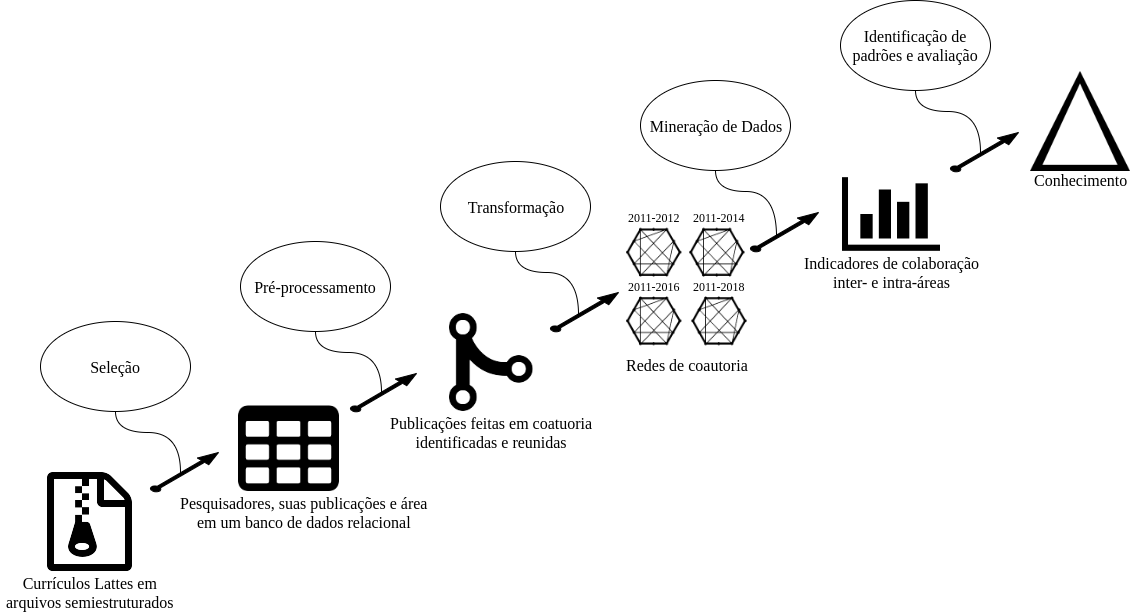
\includegraphics[scale=.3]{figuras/fayyad-diagram-graph}
  \caption{Uma visão geral dos passos adotados para o processo de descoberta de conhecimento.}
  \label{fig:processo}
\end{figure}

Este é um processo interativo e iterativo, que envolve múltiplos passos com decisões tomadas pelo pesquisador. Nas seções seguintes são discutidos os passos desse processo de descoberta de conhecimento.

\section{Seleção}

A partir de um conjunto de currículos de pesquisadores, foram extraídas informações sobre as áreas de atuação e publicações científicas, como livros, capítulos de livro, publicações em conferências e publicações em periódicos.

O \autoref{alg:selecao} apresenta o procedimento adotado, onde todos os atributos extraídos são marcados com um identificador para o currículo. Os tipos de publicações considerados neste trabalho são os livros publicados, capítulos de livro publicados, publicações completas em conferências e publicações completas em periódicos.

\begin{algorithm}
\caption{Extração de atributos do currículo do pesquisador}
\label{alg:selecao}
\begin{algorithmic}[1]

\Procedure{ExtraiaAtributos}{$id, curriculo$}
\State $A\gets \Call{SelecioneAreasDeAtuacao}{id,curriculo}$
\State $P_1\gets \Call{SelecioneLivrosPublicados}{id,curriculo}$
\State $P_2\gets \Call{SelecioneCapitulosDeLivroPublicados}{id,curriculo}$
\State $P_3\gets \Call{SelecionePublicacoesCompletasEmConferencias}{id,curriculo}$
\State $P_4\gets \Call{SelecionePublicacoesCompletasEmPeriodicos}{id,curriculo}$
\State \Return $(A,P_1,P_2,P_3,P_4)$
\EndProcedure

\end{algorithmic}
\end{algorithm}

\section{Pré-processamento}

Diversas produções científicas nessa área \cite{franceschet2011collaboration} \cite{mena2013prospecccao} \cite{reuther2006managing} descrevem casos onde uma publicação têm diversos nomes (sinônimos) e casos onde diferentes publicações possuem o mesmo nome (homônimos), cujos requerem tratamento a fim de obter um resultado mais confiável na etapa seguinte.

Neste trabalho, publicações sinônimas acontecem porque não foram cadastradas no currículo Lattes com exatamente a mesma informação, por exemplo, o mesmo título, haja vista que podem ocorrer abreviações de palavras, omissões de pontuação, ou erros de digitação.

Para amenizar este cenário foi proposto o \autoref{alg:normalizacao}, que normaliza os títulos das publicações removendo diacríticos\footnote{Um diacrítico é um sinal gráfico que se coloca sobre, sob ou através de uma letra para alterar a sua realização fonética, isto é, o seu som, ou para marcar qualquer outra característica linguística.} e elementos como tags de marcação de hipertexto, que não pertencem ao título e foram identificadas no decorrer deste trabalho.

\begin{algorithm}
\caption{Normalização do título de publicações}
\label{alg:normalizacao}
\begin{algorithmic}[1]

\Procedure{NormalizeTitulo}{titulo}
\State $titulo\gets \Call{DecodifiqueCaracteresEscapadosParaHtml}{titulo}$
\State $titulo\gets \Call{RemovaMarcacaoDeHipertexto}{titulo}$
\State $titulo\gets \Call{NormalizeParaAFormaNFKD}{titulo}$
\State $titulo\gets \Call{RemovaDiacriticosDeCaracteresASCII}{titulo}$
\State $titulo\gets \Call{NormalizeParaAFormaNFC}{titulo}$
\State \Return $titulo$
\EndProcedure

\end{algorithmic}
\end{algorithm}

Publicações homônimas são mais difíceis de ocorrer pois serão comparadas apenas publicações de um mesmo tipo referentes a um mesmo ano. Ainda, para haver o casamento entre publicações, é necessário que os títulos tenham pelo menos 3 palavras, para evitar que editoriais, por exemplo, sejam considerados uma coautoria.

Caso publicações homônimas não sejam identificadas corretamente será possível observar que a lista de coautores de um autor se dividirá em dois ou mais grupos altamente interconectados, mas sem colaborações entre grupos diferentes \cite{franceschet2011collaboration}. Ao detectar casos como este, poderá ser realizado tratamento manual.

\section{Transformação}

Usando as publicações obtidas nos currículos Lattes é possível identificar dois pesquisadores como coautores se uma mesma publicação aparece em seus currículos, e com isso construir uma rede de coautoria onde os nós são pesquisadores e os vértices a coautoria entre eles. O mesmo procedimento pode ser feito por períodos (\textit{e.g.}, biênio ou triênio), onde se obtém uma série de redes de coautoria com espaçamento temporal.

Para identificar as coautorias entre quaisquer dois autores foi proposto o \autoref{alg:coautoria}, que compara todas as publicações dentro de um mesmo ano usando o algoritmo de distância Levenshtein (\autoref{alg:levenshtein}).

\begin{algorithm}
\caption{Identificação de coautorias}
\label{alg:coautoria}
\begin{algorithmic}[1]

\Procedure{IdentificaCoautoria}{P}
\State $P^2\gets P\times{P}$
\State $C\gets \emptyset$
\ForAll{$(p_1, p_2) \in P^2$}
\If{publicações já foram comparadas}
\State \textbf{continue}
\ElsIf{publicações de anos diferentes}
\State \textbf{continue}
\ElsIf{publicações do mesmo pesquisador}
\State \textbf{continue}
\ElsIf{títulos compostos por duas palavras ou menos}
\State \textbf{continue}
\ElsIf{títulos com diferença superior a 85\% no tamanho}
\State \textbf{continue}
\ElsIf{\Call{Levenshthen}{\Call{Titulo}{$p_1$},\Call{Titulo}{$p_2$}} $<$ 0.85}
\State \textbf{continue}
\Else
\State $C\gets C\cup\{(p1, p2)\}$
\EndIf
\EndFor

\State \Return $C$
\EndProcedure

\end{algorithmic}
\end{algorithm}

\begin{algorithm}
\caption{Identificação de coautorias}
\label{alg:levenshtein}
\begin{algorithmic}[1]

\Procedure{Levenshtein}{s}
\State \Return $i$
\EndProcedure

\end{algorithmic}
\end{algorithm}

\section{Mineração de dados}

Nesta etapa serão feitos os cálculos de indicadores das redes de coautoria, onde planeja-se considerar as seguintes métricas topológicas: distância média, centralidade de grau, centralidade de proximidade, centralidade de autovetor, centralidade de contribuição, PageRank e AuthorRank\footnote{O AuthorRank é definido como uma medida que descreve as interações de um autor na rede de coautoria \cite{liu2005co}.}.

Pretendemos ainda, explorar novos arcabouços computacionais para processar todos os dados coletados.

\section{Identificação de padrões e avaliação}

Será determinada a existência de alguma correlação entre os indicadores obtidos e a análise desses indicadores para determinar se existe influência (ou impacto relativo) da Ciência da Computação em outras áreas.

Complementarmente, acontecimentos históricos que possam justificar o padrão encontrado serão buscados a fim de contextualizar a avaliação.

Diferentes conceitos de aprendizado de máquina e reconhecimento estatístico de padrões serão abordados.

\chapter{Resultados e Discussão}

Nesta seção apresentamos os resultados obtidos a partir da análise das coautorias, onde são discutidos os resultados relacionados à produção bibliográfica, impacto e colaboração com as demais áreas e a interdisciplinaridade da Ciência da Computação, comparando-a com as demais áreas e discutindo como suas relações acontecem sob o ponto de vista das coautorias.

\section{Produção bibliográfica}

O número de publicações científicas únicas feitas em coautoria com pesquisadores da Ciência da Computação é de $282.796$, sendo a 5ª área que mais colabora considerando as publicações de todos os tempos, ficando atrás apenas da Medicina, Agronomia, Educação e Química, como mostra a \autoref{tab:producaoporarea}.

\begin{table}[htpb]
    \centering
    \caption{As 10 áreas que mais produzem publicações científicas em coautoria na ciência brasileira.}
    \label{tab:producaoporarea}
    \begin{tabular}{|r|l|c|}%
        \hline & Área & Número de publicações\\\hline
        \csvreader[late after line=\\\hline]%
        {"tabelas/resultados-producao-bliografica-por-area.csv"}%
        {area=\area,contagem=\contagem}%
        {\thecsvrow & \area & \contagem}%
    \end{tabular}
\end{table}

A \autoref{fig:coautoriaanual} apresenta um gráfico de segmento anual, que vai do ano de surgimento do Currículo Lattes até o último ano completo, com o crescimento do número de publicações feitas em coautoria das áreas que mais produzem em coautoria. Nele é possível observar que o crescimento do número de coautorias da Ciência da Computação não foi alto, e acompanhou as demais áreas do conhecimento consideradas.

São exceções as áreas de Educação e Medicina, que durante os períodos de 2004-2009 e 2002-2006, respectivamente, tiveram crescimento acelerado e depois se mantiveram estáveis. Ainda, é importante pontuar que existe uma queda acentuada em todas as áreas no ano de 2018, mas isso está provavelmente relacionado ao fato da coleta ter sido feita em janeiro de 2019 e as publicações do ano de 2018 não terem sido todas concluídas.

\begin{figure}[htpb]
  \centering
  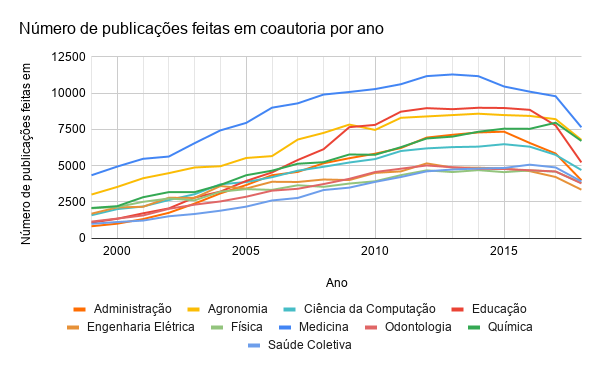
\includegraphics[width=1\textwidth]{figuras/resultados-grafico-coautoria-anual}
  \caption{Gráfico de segmento anual com a produção em coautoria das áreas que mais produzem em coautoria no período de 1999 a 2018.}
  \label{fig:coautoriaanual}
\end{figure}

\section{Impacto e colaboração}

A rede de colaboração entre as áreas apresentada na \autoref{fig:grafocolaboracao} foi construída a partir da rede de coautoria entre os pesquisadores. O diâmetro da rede é igual a $3$, o caminho médio igual a $1,31$ e coeficiente médio de clusterização igual a $0,912$. Essa rede apresenta um comportamento comumente observado em redes sociais, é coesa e se caracteriza pela alta densidade de arestas, indicando que quase todas as áreas do conhecimento estão relacionadas entre si. Este fato observado se comporta como o esperado, dado que na ciência não se trabalha de forma isolada.

\begin{figure}[htpb]
  \centering
  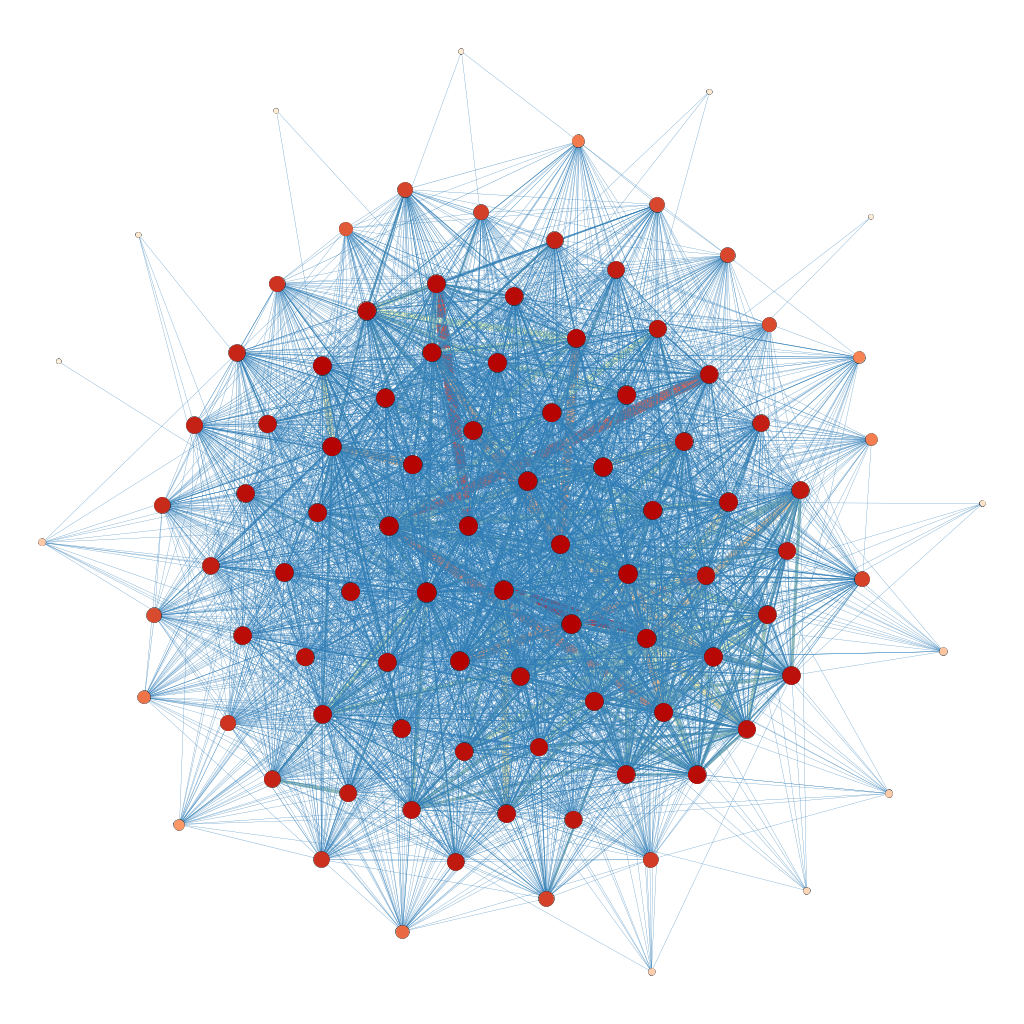
\includegraphics[width=1\textwidth]{figuras/resultados-grafo-colaboracao-entre-areas}
  \caption{Grafo de colaboração entre as áreas do conhecimento.}
  \label{fig:grafocolaboracao}
\end{figure}

O mapa de calor obtido na \autoref{fig:mapadecalorcolaboracao}, com a colaboração exercida entre as áreas, mostra que o maior esforço de colaboração da Ciência da Computação está com a Engenharia Elétrica, sendo que as áreas mais impactadas pela Ciência da Computação são a Matemática, Engenharia Elétrica e Ciência da Informação. Ainda segundo este mapa, podemos ver que a Medicina é a área que mais impacta áreas distintas.

\begin{landscape}
  \begin{figure}[htbp]
    \centering
    \includegraphics[width=\linewidth, height=\textheight, keepaspectratio]%
    {figuras/resultados-mapa-de-calor-colaboracao-entre-areas}
    \caption{Mapa de calor das colaborações exercidas entre as áreas. As linhas horizontais podem ser interpretadas como o impacto exercido e as linhas verticais podem ser entendidas como a relevância que outra área recebeu esse impacto.}
    \label{fig:mapadecalorcolaboracao}
  \end{figure}
\end{landscape}

Uma visualização que permite observar o impacto exercido por cada área é apresentada na \autoref{fig:grafoimpacto}, uma interpretação do mesmo mapa de calor, onde os nós são as áreas do conhecimento e as arestas direcionadas representam o impacto que é exercido pela área, isto é, quanto das suas colaborações determinam as produção científica feita em colaboração das outras áreas.

Nele é possível observar que existem $7$ componentes conexas, a maior componente conexa conta com 61 nós, o que representa $62,89$\% da rede. A Ciência da Computação faz parte de um subgrafo que está interconectado pela Engenharia da Computação, onde pode ser visto que de fato o impacto é relevante apenas na Engenharia Elétrica.

\begin{figure}[htpb]
  \centering
  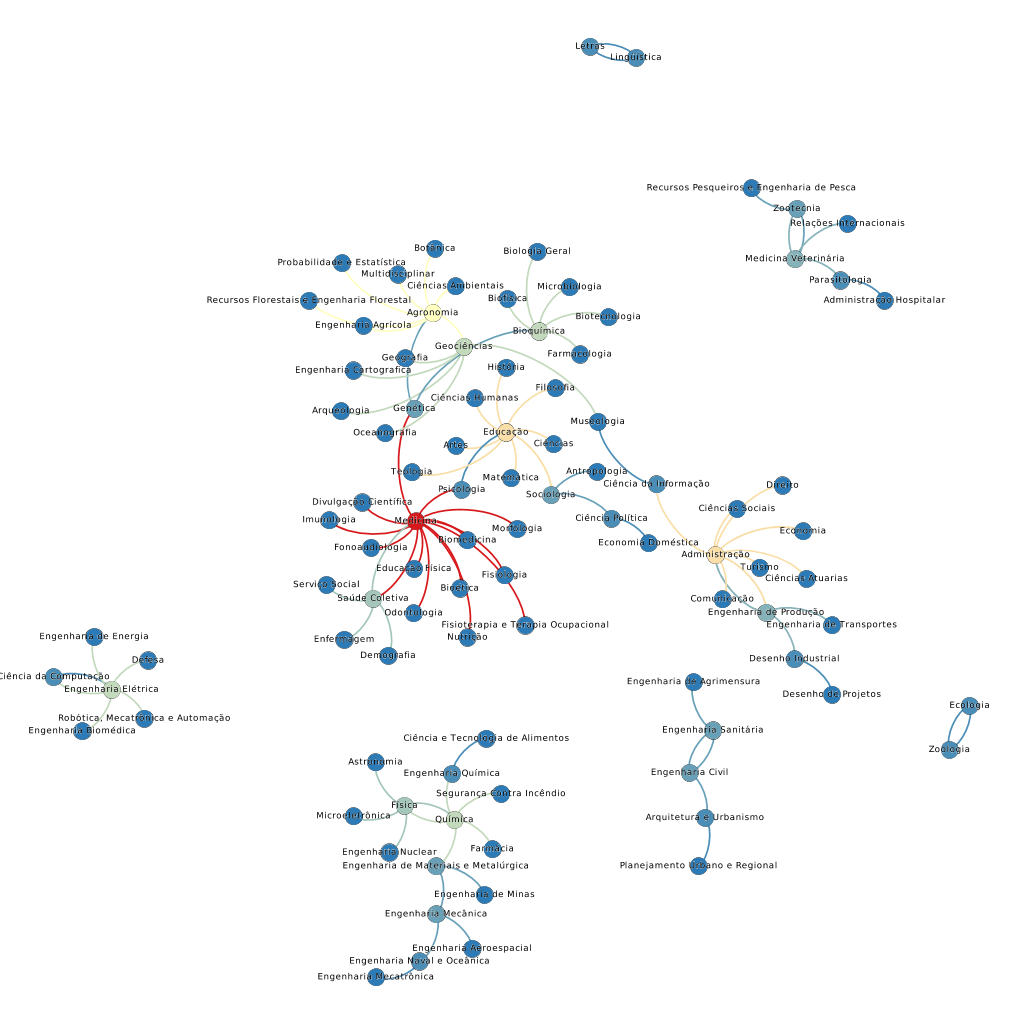
\includegraphics[width=1\textwidth]{figuras/resultados-grafo-impacto}
  \caption{Grafo do impacto exercido pela área na produção científica feita em colaboração das outras áreas. Os nós com cores mais quentes são os que mais exercem impacto em outras áreas.}
  \label{fig:grafoimpacto}
\end{figure}

\section{Interdisciplinaridade}

Interdisciplinaridade é um conceito que pode ser interpretado de diferentes maneiras. Neste trabalho uma publicação em coautoria será considerada interdisciplinar se os coautores pertencem a pelo menos 3 áreas distintas.

O número de publicações científicas interdisciplinares feitas em coautoria apresentado na \autoref{tab:producaointerdisciplinar} mostra que a Ciência da Computação, apesar de construir muitas publicações em coautoria, não tem muita atuação em projetos desse tipo.

\begin{table}[htpb]
    \centering
    \caption{As 20 áreas com o maior número de publicações interdiscplinares.}
    \label{tab:producaointerdisciplinar}
    \begin{tabular}{|r|l|c|}%
        \hline & Área & Número de publicações interdisciplinares\\\hline
        \csvreader[late after line=\\\hline]%
        {"tabelas/resultados-producao-bibliografica-interdisciplinar.csv"}%
        {area=\area,contagem=\contagem}%
        {\thecsvrow & \area & \contagem}%
    \end{tabular}
\end{table}

A Medicina aparece como a área com mais publicações feitas em grupos interdisciplinares, são $37.578$ das suas $565.761$ publicações feitas em coautoria. Todavia, este número ainda representa pouco mais de $6,5$\% das publicações.

Podemos ver na \autoref{tab:producaogrupointerdisciplinar} que a maioria das publicações da Ciência da Computação feitas em coautoria são feitas com uma área do conhecimento distinta, o que mostra que publicações interdisciplinares não são muito comuns. Isso também é observado na Medicina, Educação, Agronomia e Administração, o que sugere ser um comportamento comum. 

\begin{table}[htpb]
    \centering
    \caption{Número de publicações onde os grupos com pesquisadores Ciência da Computação eram compostos por pesquisadores de outras áreas.}
    \label{tab:producaogrupointerdisciplinar}
    \begin{tabular}{|r|r|}%
        \hline Número áreas & Contagem de publicações \\\hline
        \csvreader[late after line=\\\hline]%
        {"tabelas/resultados-producao-bibliografica-computacao-e-grupos-interdisciplinares.csv"}%
        {tamanhodogrupo=\tamanhodogrupo,contagem=\contagem}%
        {\tamanhodogrupo & \contagem}%
    \end{tabular}
\end{table}

\chapter{Considerações finais}

A ciência da computação é uma área que se conecta a quase todas as áreas do conhecimento que apareceram em nossa listagem, porém não exerce impacto significativo em suas produções bibliográficas. Isso contradiz a sensação de que a computação está envolvida em tudo nos dias de hoje.

Poderíamos dizer que os produtos da ciência da computação são bastante usados em nosso dia a dia e com certeza também nas pesquisas de outras áreas, porém profissionais da área não são requisitados para os estudos. Sendo assim, poderíamos apenas dizer que talvez os produtos da ciência da computação permeiem tudo e tenham impacto na pesquisa, mas não podemos dizer que a pesquisa realizada no brasil envolve pesquisadores da área.

Análises de caso de pesquisas que aconteceram poderiam ser feitas para entender qual o papel exercido pela ciência da computação nessas outras áreas e entender se é apenas o volume que é baixo.

\section{Limitações}

A base de dados é um retrato do mês de janeiro de 2019, e não ter os dados atualizados de forma mais ágil é um fator que dificulta a descoberta do conhecimento, acompanhando a mudança que acontece dia após dia.

Ainda, o processamento durou cerca de duas 1 semana e meia, o que significa dizer que se um novo retrato fosse feito hoje não conseguiríamos disponibilizar em tempo hábil.

O algoritmo usado para comparação dos título é $O(n^2)$ o que significa dizer que ele é quadrático em relação ao número de entrada. Os filtros aplicados de ano e similaridade por diferença de tamanho da string ajudam a diminuir o tempo de execução, mas não é suficiente.

Nem todos os pesquisadores preenchem suas áreas e isso faz com que tenhamos que desconsiderar boa parte dos dados. Assim, temos dados desconhecidos que não sabemos inferir sua área de atuação. Apesar de termos informações sobre a formação do pesquisador, não extraímos esse dado do currículo e portanto não conseguimos usá-lo.

As análises estão pouco aprofundadas porque muito tempo foi investido no processamento dos dados e outras estratégias que foram aplicadas no passado fizeram o tempo ser mal investido. Houveram problemas com servidores. Mudança de ferramentas, gastos com computação em nuvem para auxiliar no processamento.

\section{Trabalhos futuros}

Existem muitas análises que podem ser derivadas do banco de dados construído, uma vez que ele dá o panorama geral das coautorias de todos os pesquisadores com nível de instrução de doutorado na plataforma lattes. Com os dados já presentes no banco de dados é possível entender como funcionam as coautorias entre as universidades, possibilitando entender qual é o nível de interação entre elas. Também é possível entender como anda a produção de materiais de divulgação científica, dado que esse indicador também foi coletado.

Também poderiam ser considerados estudos sobre a rede de coautoria, explorando suas propriedades, identificando os pesquisadores mais produtivos e mais influentes na comunidade científica brasileira. Foi observado por ena-chalco que os autores mais produtivos são os que mais colaboram, e um estudo dos assuntos abordados nessas colaborações também poderia ser feito aplicando técnicas de processamento de linguagem natural no título das publicações.

Pode ser construída uma ferramenta capaz de desambiguar autores. É um problema identificar todos os coautores de uma publicação em citações, pois muitas delas apresentam apenas o nome do primeiro pesquisador com o et. al.. A partir apenas do título da publicação e o ano poderíamos fornecer a lista completa de pelo menos os pesquisadores presentes na plataforma lattes.

Poderíamos explorar a produção por nível acadêmico e entender como grandes pesquisadores trabalharam em coautoria, o que poderia indicar que a evolução da ciência se dá por essas relações.
% \chapter{Limitações}

% %\chapter{Trabalhos futuros}


% ----------------------------------------------------------
% ELEMENTOS PÓS-TEXTUAIS (Referências, Glossário, Apêndices)
% ----------------------------------------------------------
\postextual

% Referências bibliográficas
\bibliography{bibliografia}

% Glossário (Consulte o manual)
%\glossary

% Apêndices
% ----------------------------------------------------------
% Apêndices
% ----------------------------------------------------------

% ---
% Inicia os apêndices
% ---
\begin{apendicesenv}

% Imprime uma página indicando o início dos apêndices
\partapendices

% ----------------------------------------------------------
\chapter{Primeiro Apêncice}
% ----------------------------------------------------------

\lipsum[50] % Texto qualquer. REMOVER!!

% ----------------------------------------------------------
\chapter{Segundo apêndice com título tão grande quanto se queira porque ele já faz a quebra de linha da coisa toda}
% ----------------------------------------------------------
\lipsum[51-53] % Texto qualquer. REMOVER!!

\end{apendicesenv}
% ---

% Anexos
% % ----------------------------------------------------------
% Apêndices
% ----------------------------------------------------------

% ---
% Inicia os anexos
% ---
\begin{anexosenv}

% Imprime uma página indicando o início dos anexos
\partanexos

% ---
\chapter{Nome do Primeiro Anexo}
% ---

% ---
\chapter{Nome de Outro Anexo}
% ---

\end{anexosenv}

% Índice remissivo (Consultar manual)
%\phantompart
%\printindex

\end{document}
